\documentclass{article}

\pdfoutput=1

\usepackage{amsmath}
\usepackage{amsfonts}
\usepackage{mathtools}
\usepackage{graphicx}
\usepackage[margin=1in]{geometry}

\graphicspath{{figures/}}

\title{A Tool for Visualizing and Analyzing High-Dimensional Clustering Performance}
\author{Justin Lin\footnote{Department of Mathematics, Indiana University} and Julia Fukuyama\footnote{Department of Statistics, Indiana University}}
\date{}

\begin{document}
\maketitle

\abstract{Technological advances have spurred an increase in data complexity and dimensionality. We are now in an era in which data sets containing thousands of features are commonplace. To digest and analyze such high-dimensional data, dimension reduction techniques have been developed and advanced along with computational power. Of these techniques, nonlinear methods are most commonly employed when working with high-dimensional data because of their ability to construct visual two-dimensional embeddings of high-dimensional data. These methods unevenly stretch and shrink space in a way that represents the data's structure in a fewer number of dimensions. However, attempting to capture high-dimensional structures in a significantly lower number of dimensions requires drastic manipulation of space. As such, nonlinear dimension reduction methods are known to occasionally capture false structures, especially in noisy settings. In efforts to deal with this phenomenon, we developed an interactive tool that enables analysts to better understand and diagnose their dimension reduction results. It uses various analytical plots to provide a multi-faceted perspective on captured structures in the data to determine if they're faithful to the original data or remnants of the dimension reduction process. The tool is available in an R package named \textit{insert name here}.}

\section{Introduction}
The potency of nonlinear dimension reduction methods lies in their flexibility, allowing them to model complex data structures. That same flexibility, however, makes them difficult to use and interpret. Each method requires a slew of hyperparameters that need to be calibrated, and even when adequately calibrated, these methods require a trained eye to interpret. For example, the two most popular nonlinear dimension reduction methods, t-SNE and UMAP, are known to generate unintuitive results (\cite{understanding UMAP}, \cite{Distill}). The results often cluster, even when no clusters exist in the data. Moreover, cluster sizes and inter-cluster distances can be unreliable. We've developed an interactive tool that analysts may use to conduct a post-hoc analysis of their high-dimensional clustering. The tool uses the minimum spanning three (MST) to model the global structure of clusters and to provide an additional perspective on inter-cluster relationships. This allows analysts to extract more information from their dimension reduction results by making it easier to differentiate the signal and the noise.

\section{Methods}

\subsection{The Minimum Spanning Tree}
Graphs have been applied to many multivariate statistical problems. The authors of \cite{MAP test} introduced the minimal ascending path spanning tree as a way to test for multimodality. The Friedman-Rafsky test \cite{Friedman-Rafsky test}, along with its modern variations \cite{Friedman-Rafsky variation 1, Friedman-Rafsky variation 2, Friedman-Rafsky variation 3}, use the MST to construct a multivariate two-sample test. Single-linkage clustering \cite{single-linkage and MST} and runt pruning \cite{runt pruning} are both intimately related with the MST. In the context of dimension reduction, IsoMap \cite{IsoMap} makes use of neighborhood graphs, \cite{MIST example} introduces the maximum information spanning tree, and \cite{MST example} uses the MST. These methods, which fall under the category of manifold learning, use graphs to model high-dimensional data assumed to be drawn uniformly from a non-linear manifold. An accurate low-dimensional embedding can then be constructed from these graphs. It's apparent that graphs are useful for modeling high-dimensional data, especially when it comes to dimension reduction and cluster analysis. Our tool uses the MST to analyze the reliability of visualizations produced by nonlinear dimension reduction methods.

To construct the minimum spanning tree (MST) from a data set, start with a set of vertices, one for each point in the data set. When an edge is added between two vertices, its assigned a weight equal to the dissimilarity between the pair of points corresponding to the two vertices. The edges of the MST are selected from all possible edges so that the sum of edge weights is minimized and there exists a path between any two vertices. We've opted for the MST for a couple of key properties. Firstly, the MST and shortest paths along it are quick to compute. Secondly, the MST contains a unique path between any two vertices, providing inter-point distances between all pairs of points. Lastly, it provides a good summary of the data's structure. It contains as a subgraph the nearest-neighbor graph, and any edge deletion in the MST partitions the vertices into two sets for which the deleted edge is the shortest distance between them \cite{Friedman-Rafsky test}.

\subsection{The Inputs}
The interactive tool takes as input a dissimilarity matrix $D \in \mathbb{R}^{n \times n}$ representing the dissimilarities between the $n$ high-dimensional points, a two-dimensional embedding $X \in \mathbb{R}^{n \times 2}$, and a clustering $\mathcal{C} \in \{1, \hdots, k\}^n$ where $k$ is the number of classes. Optionally, it also takes a set of ID's to denote the points.

The dissimilarity matrix must be a symmetric matrix with 0's along the diagonal. The entry $D_{ij} = D_{ji}$ should represent the dissimilarity or distance between points $i$ and $j$. The chosen dissimilarity measure should be appropriate for the type of data. For example, the $L_1$ norm and even fractional $L_p$ distance measures have been suggested for high-dimensional numerical data \cite{fractional Lp norms}, Jaccard and cosine metrics are popular when working with text data \cite{text data}, and a variety of Image Distance Functions (IDFs) have been suggested for image data \cite{image metrics}. From this dissimilarity matrix, the MST is calculated.

\subsection{The Dashboard}

\renewcommand{\figurename}{Figures}
\renewcommand{\thefigure}{1a and 1b}
\begin{figure}[t]
\centering
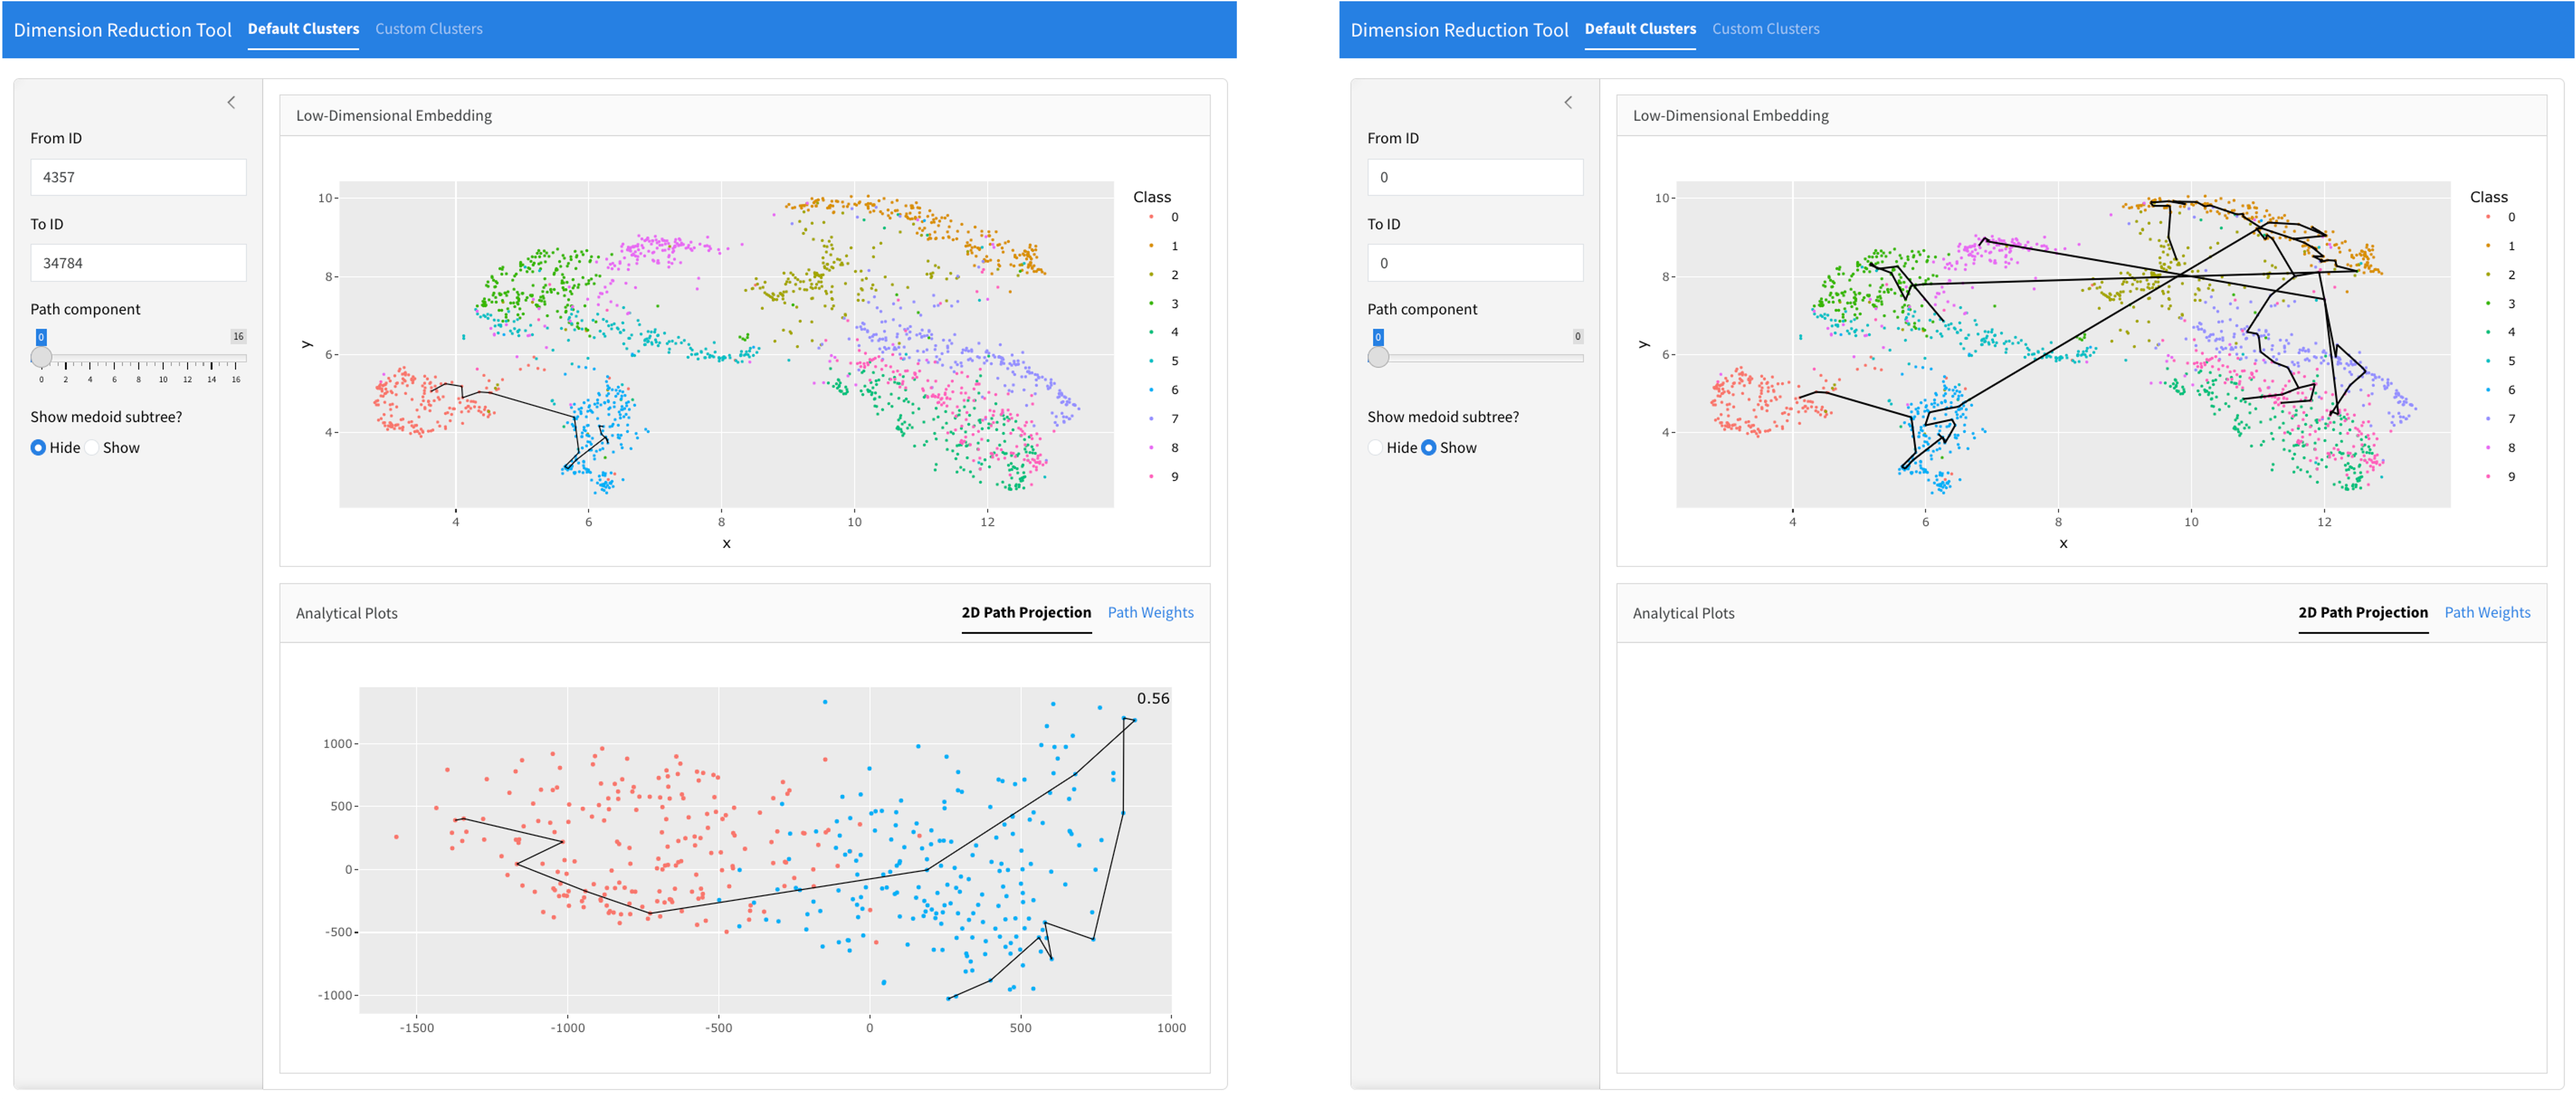
\includegraphics[scale=0.47]{dashboard}
\caption{Dashboard}
\end{figure}

The dashboard contains two main panels, as well as a side panel include adjustable settings. The first main panel depicts the low-dimensional embedding colored according to the provided clustering. The second main panel contains analytical plots. When supplied with a pair of points via ``From ID" and ``To ID", the MST path is calculated between the high-dimensional points and corresponding path in low-dimension is drawn upon the low-dimensional embedding (Figure 1a). The first analytical plot depicts a PCA projection of the high-dimensional path along with the clusters the two endpoints belong to. The PCA transform is calculated using only the points along the path then applied to the rest of the points. The number in the top right corner is the proportion of variance retained by the PCA projection. The second analytical plot contains a bar plot of path weights. The user may cycle through the segments along the path using the ``Path component" slider in the side panel. The corresponding segment will be highlighted in both the low-dimensional embedding and the 2D path projection. The corresponding path weight will also be highlighted in the plot of path weights.

To get a holistic view of the data's structure, the user may view the medoid subtree by selecting ``Show" in the side panel (Figure 1b). The medoid subtree is the minimal subtree of the MST containing the medoid of each class. The medoid subtree describes the global arrangement of clusters.

Along the top bar, the user may also navigate to the next page named ``Custom Clusters". This page contains the same plots, but the user may instead define their own clusters of interest. To define a cluster, the user must select a subset of points by clicking and dragging along the low-dimensional embedding plot. Once the points are selected, the user can save the selected points by clicking ``Submit Group 1". The user must then repeat the process with the second cluster of points and click ``Submit Group 2". Once both clusters have been submitted, the path between the (high-dimensional) medoids of the selected clusters is portrayed. The 2D path projection will contain the points along the path together with the selected points. This page is highly useful for analyzing spacial clusters that may not be represented by the provided clustering.

\section{Results}
In this section, we walk through a few examples to demonstrate how to use the tool effectively.

\subsection{MNIST}
The MNIST database is a collection of 70,000 images of handwritten digits \cite{MNIST}. Each image contains 784 x 784 pixels, so when vectorized, the data set contains 70,000 points in 614,656 dimensions. A random subsample of 2,000 images was taken and PCA pre-processing step was applied. The number of dimensions was reduced to 300 before applying UMAP to construct a two-dimensional visualization.

\renewcommand{\figurename}{Figure}
\renewcommand{\thefigure}{2}
\begin{figure}[t]
\centering
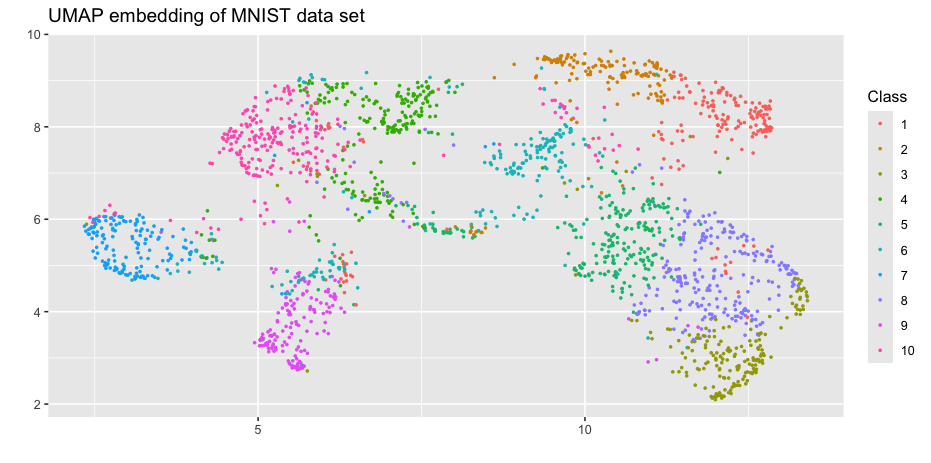
\includegraphics[scale=0.43]{MNIST kmeans}
\caption{UMAP embedding of MNIST data set (k-means clustering)}
\end{figure}

 To demonstrate how to use the tool, we analyze a hypothetical clustering instead of the true class labels. k-means was applied to the pre-processed data with 10 clusters,  one for each digit. It is immediately evident that k-means does not agree with the UMAP embedding for some clusters.
 
 \subsubsection{Upper Right Cluster}
 
Let's begin by investigating the cluster in the upper right corner of the plot. k-means is known to struggle with clusters of varying sizes and densities, so this cluster may have been incorrectly split into two distinct classes (orange and red).

\renewcommand{\figurename}{Figures}
\renewcommand{\thefigure}{3a, 3b, 3c}
\begin{figure}[t]
\centering
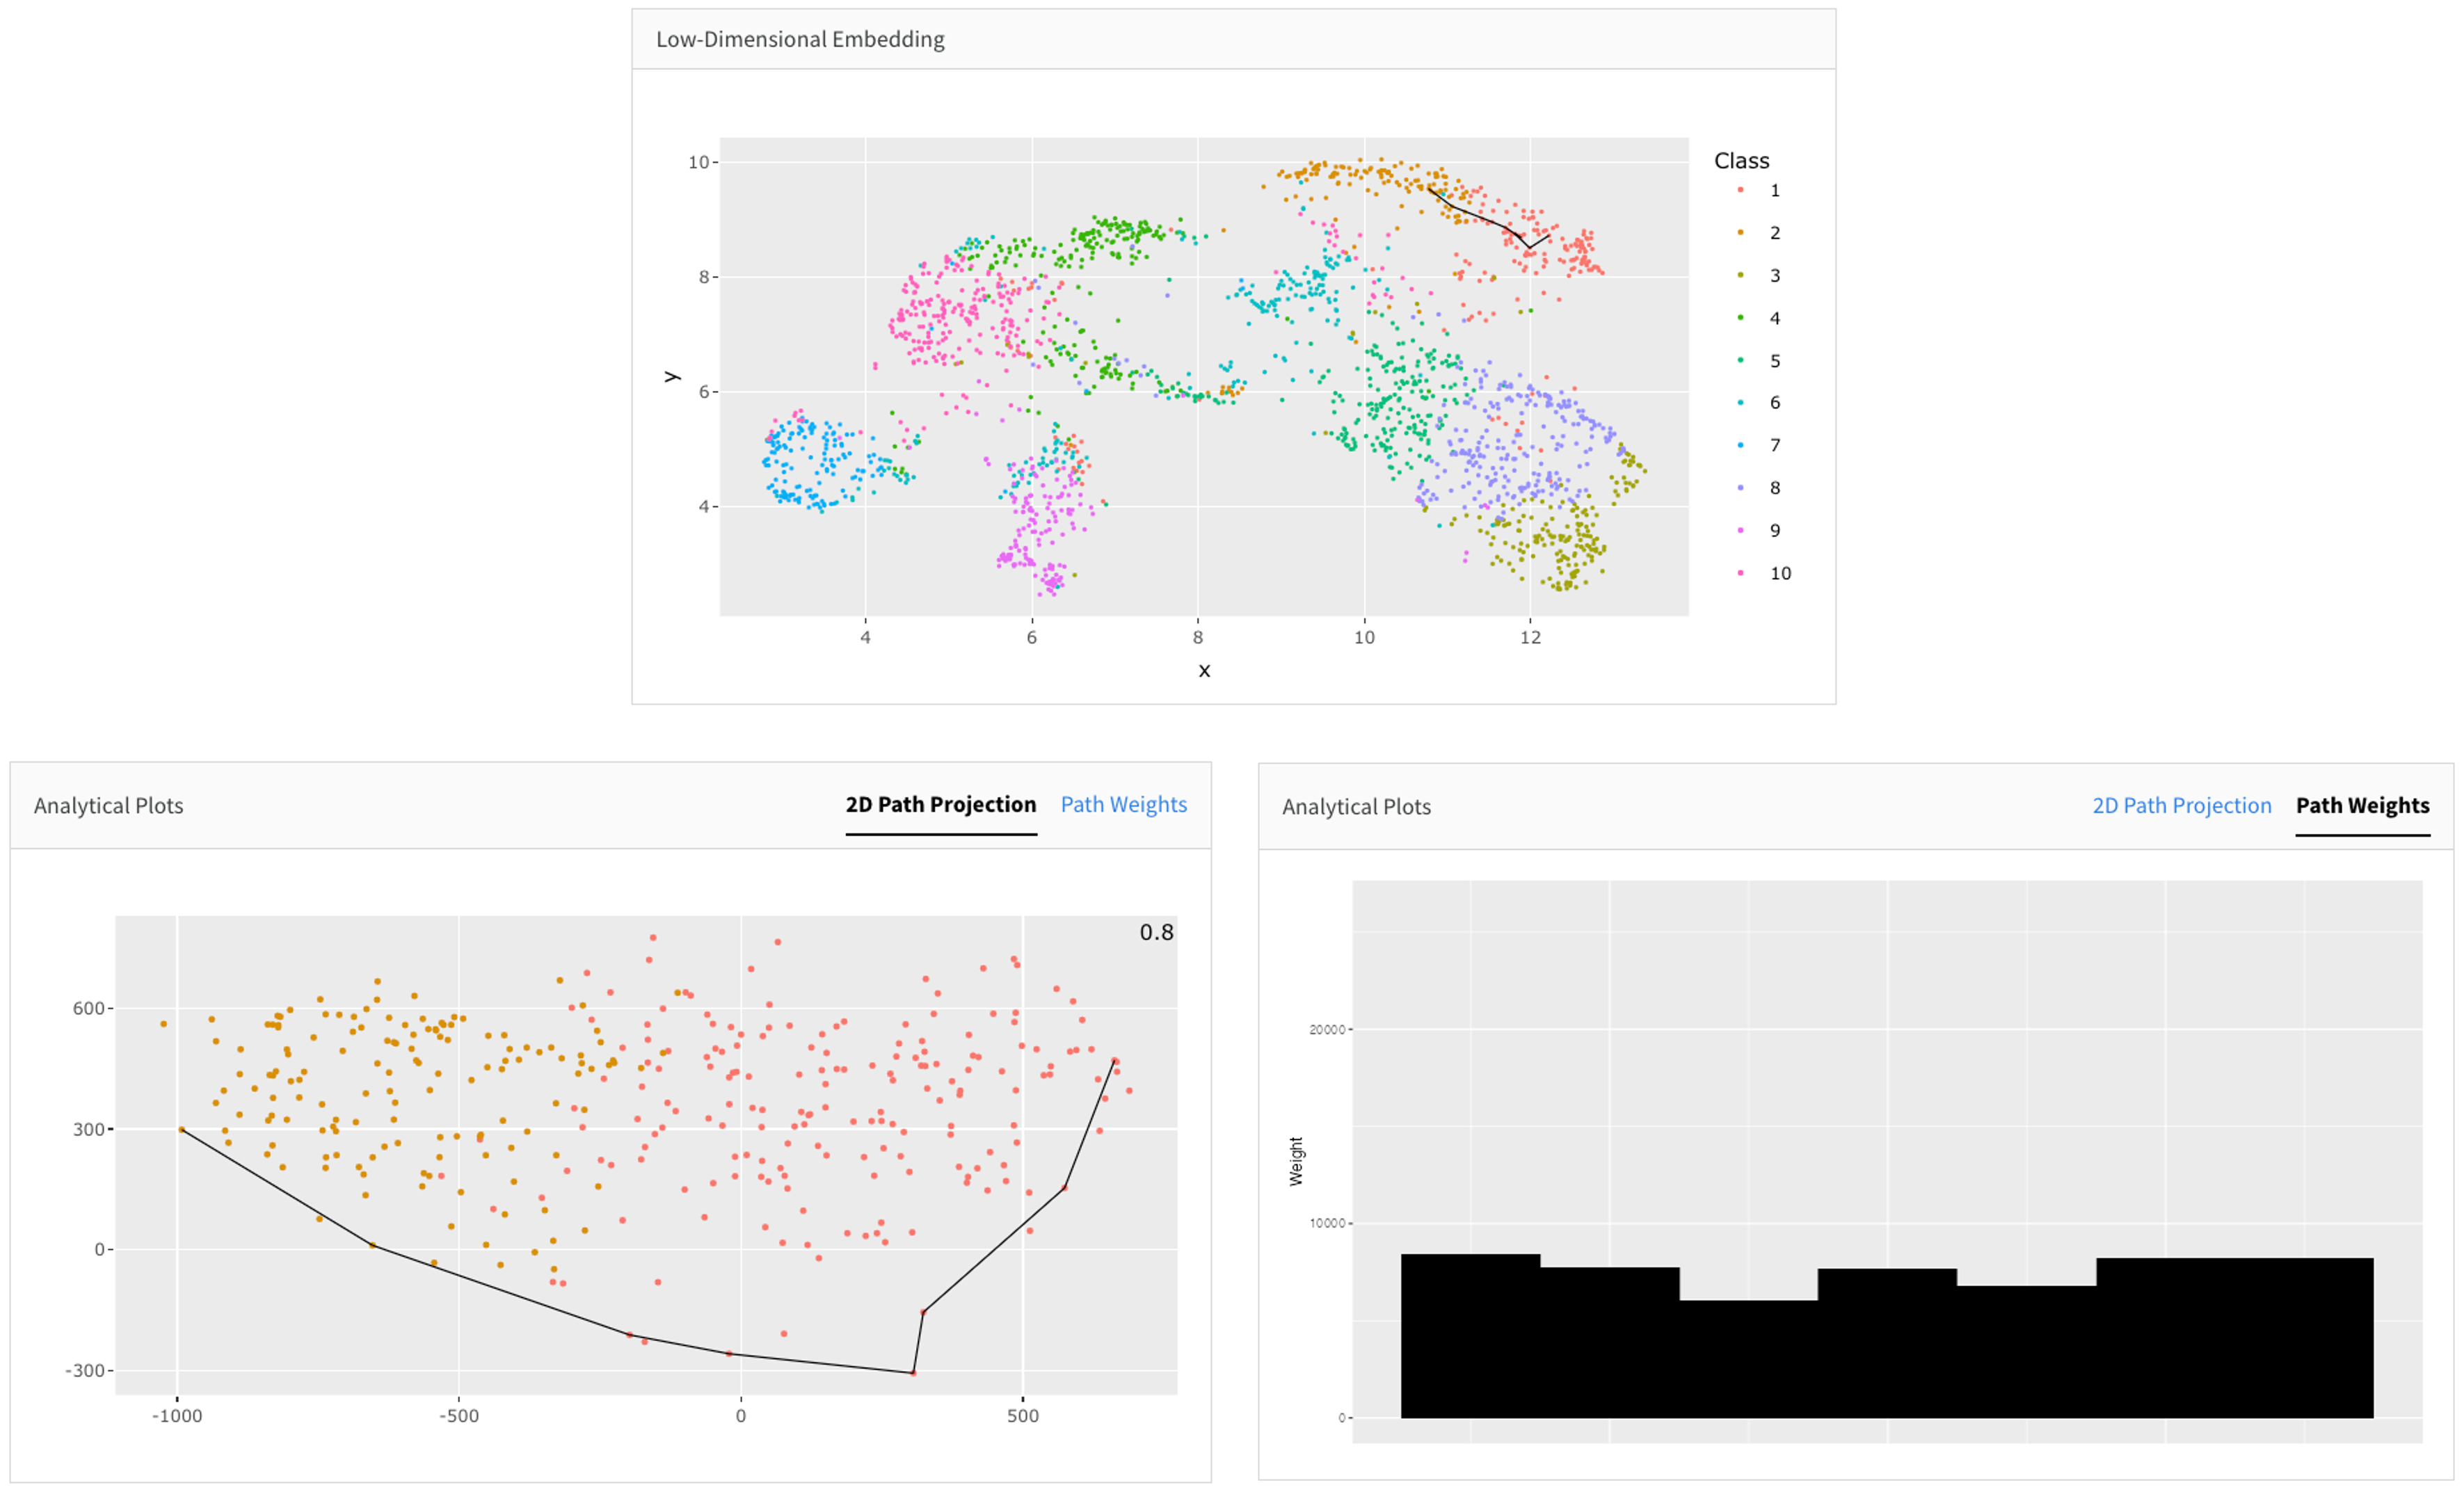
\includegraphics[scale=0.5]{MNIST (orange red)}
\caption{Path between upper right clusters (MNIST)}
\end{figure}


 
\newpage

\begin{thebibliography}{10}

\bibitem{fractional Lp norms}
Charu C. Aggarwal, Alexander Hinneburg, and Daniel A. Keim.
\newblock On the surprising behavior of distance metrics in high dimensional space.
\newblock {\em Lecture Notes in Computer Science, vol. 1973}, 2001.

\bibitem{Friedman-Rafsky variation 1}
Bhaswar B. Bhattacharya.
\newblock A general asymptotic framework for distribution-free graph-based two-sample tests.
\newblock {\em Journal of the Royal Statistical Society Series B: Statistical Methodology 81:3, 575-602}, 2019.

\bibitem{Friedman-Rafsky variation 2}
Hao Chen and Jerome H. Friedman.
\newblock A new graph-based two-sample test for multivariate and object data.
\newblock {\em Journal of the American Statistical Association 112:517, 397-409}, 2017.

\bibitem{Friedman-Rafsky variation 3}
Hao Chen, Xu Chen, and Yi Su.
\newblock A weighted edge-count two-sample test for multivariate and object data.
\newblock {\em Journal of the American Statistical Association 113:523, 1146-1155}, 2018.

\bibitem{understanding UMAP}
Andy Coenen and Adam Pearce for Google PAIR.
\newblock Understanding UMAP.
\newblock {\em https://pair-code.github.io/understanding-umap/}.

\bibitem{MNIST}
Li Deng.
\newblock The MNIST database of handwritten digit images for machine learning research.
\newblock {\em IEEE Signal Processing Magazine 29:6}, 2012.

\bibitem{image metrics}
Vito Di Ges\`u and Valery Starovoitov.
\newblock Distance-based functions for image comparison.
\newblock {\em Pattern Recognition Letters 20:2, 207-214}, 1999

\bibitem{single-linkage and MST}
J. C. Gower and G. J. S. Ross.
\newblock Minimum spanning trees and single linkage cluster analysis.
\newblock {\em Journal of the Royal Statistical Society. Series C (Applied Statistics) 18:1, 54-64}, 1969.

\bibitem{Friedman-Rafsky test}
Jerome H. Friedman and Lawrence C. Rafsky.
\newblock Multivariate generalizations of the Wald-Wolfowitz and Smirnov two-sample tests.
\newblock {\em Annals of Statistics 7:4, 697-717}, 1979.

\bibitem{MIST example}
Bracken M. King and Bruce Tidor.
\newblock MIST: Maximum information spanning trees for dimension reduction of biological data sets.
\newblock {\em Bioinformatics 25:9, 1165-1172}, 2009.

\bibitem{text data}
Abdul Wahab Qurashi, Violeta Holmes, and Anju P. Johnson.
\newblock Document processing: Methods for semantic text similarity analysis.
\newblock {\em IEEE}, 2020.

\bibitem{runt pruning}
Werner Stuetzle.
\newblock Estimating the cluster tree of a density by analyzing the minimal spanning tree of a sample.
\newblock {\em Journal of Classification 20, 25-47}, 2003.

\bibitem{IsoMap}
Joshua B. Tenenbaum, Vin de Silva, and John C. Langford.
\newblock A global geometric framework for nonlinear dimensionality reduction.
\newblock {\em Science 290:2319}, 2000.

\bibitem{MST example}
Daniel Probst and Jean-Louis Reymond.
\newblock Visualization of very large high-dimensional data sets as minimum spanning trees.
\newblock {\em Journal of Cheminformatics 12:12}, 2020.

\bibitem{MAP test}
Gregory Paul M. Roz\'al and J.A. Hartigan.
\newblock The MAP test for multimodality.
\newblock {\em Journal of Classification 11, 5-36}, 1994.

\bibitem{Distill}
Martin Wattenberg, Fernanda Vi\'egas, and Ian Johnson.
\newblock How to Use t-SNE Effectively.
\newblock {\em Distill}, 2016.

\end{thebibliography}

\end{document}